

\documentclass{standalone}
\usepackage{pgfplotstable}
\pgfplotsset{compat=1.12}

\begin{document}
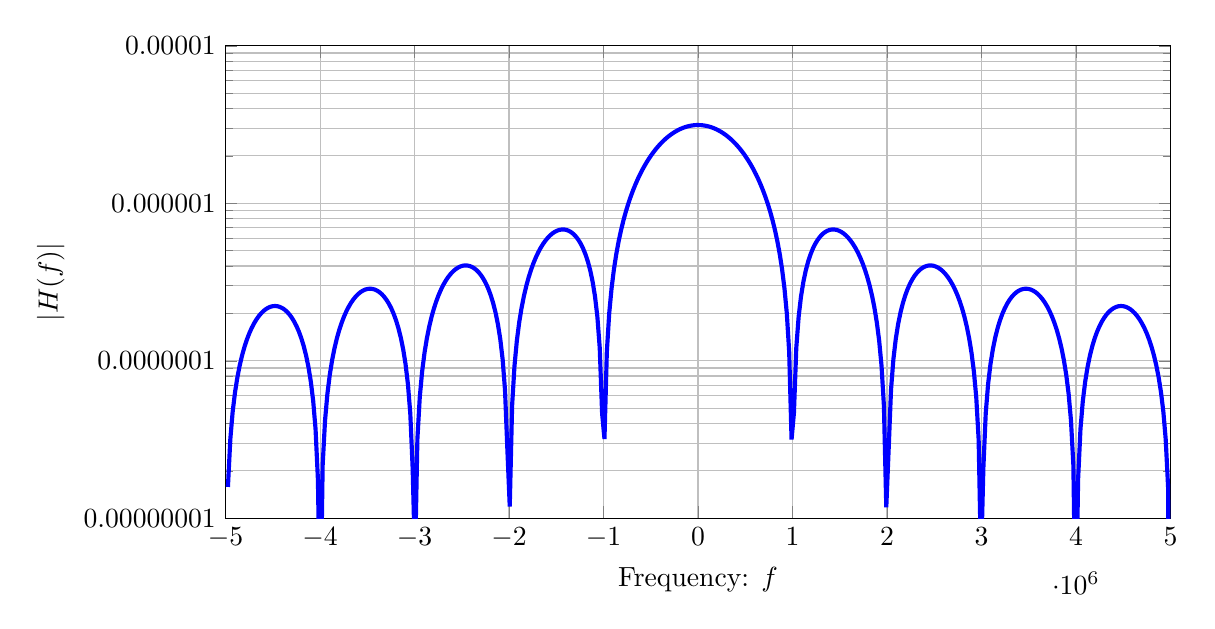
\begin{tikzpicture}
    \begin{semilogyaxis}
        [
           log ticks with fixed point,
           width=12.0cm,
           height=6cm,
            scale only axis,
            xmin=-5e6, xmax=5e6,
            ymin=1e-8, ymax=1e-5,
            grid=both,
            domain=-5e6:5e6,
            samples=400,
            xlabel={Frequency: $f$},
           ylabel={$|H(f)|$},
           % label style={% erst nach Option axis lines verwenden
           %  at={(ticklabel cs:0.5)},anchor=near ticklabel,sloped},
        ]
        \addplot+[mark=none, line width = 1.5] {1e-6*abs(sin(deg(x*pi*1e-6))/(x*1e-6)}; 
    \end{semilogyaxis}        
\end{tikzpicture}
\end{document}